\documentclass{article}
\usepackage[utf8]{inputenc}
\usepackage[hyphens]{url} 
\usepackage[breaklinks]{hyperref}
\usepackage{amsmath,amsthm,stmaryrd,amssymb,fdsymbol}
\usepackage{bussproofs}
\usepackage{listings}
\usepackage{tikz}

\newtheorem{theorem}{Theorem}[section]
\newtheorem{definition}{Definition}[theorem]

\newcommand{\la}{^{\leftarrow}}
\newcommand{\ra}{^{\rightarrow}}
\newcommand{\refl}{\hourglass}

\title{Security-Typed Languages \\ \Large{Lecture 4}} 

\begin{document}

\maketitle

\section{Transparent Endorsement}

From last time: NI $\rightarrow$ Robust declassification (NI refines RD). Robust declassification breaks the confidentiality/integrity duality.

To restore duality define
Transparent Endorsement (TE).
% figure 1 here
Example: password checker
\begin{lstlisting}[mathescape,frame=single,basicstyle=\ttfamily,language=java]
String{H} pwd;
 bool{H$^{\leftarrow}$} check_password(String{H$^{\rightarrow}$} guess) {
    String{H} endorsed_guess = endorse(guess,H$^\rightarrow$ to H);
    bool{H} res = (password == endorsed_guess);
    return declassify(res,H to H$^{\leftarrow}$);
}
\end{lstlisting}
A problem can arise when adversary manages to steer password value directly into \texttt{check\_password} function, abusing downgrading. The problem arises because \texttt{pwd} with H label (trusted) can flow into H$^{\rightarrow}$ (untrusted). To solve the problem we can give label L to variable $\texttt{guess}$ (untrusted and unconfidential).

This is enforced by the typing  rule for \emph{transparent endorsement}:

\begin{prooftree}
    \AxiomC{$\Gamma(y) \sqsubseteq l_1$}
    \AxiomC{$ l_2 \sqsubseteq\Gamma(y) $}
    \AxiomC{$ l_1 \sqsubseteq l_2 \sqcup \bigtriangledown (l_1 \sqcup pc) $}
    \TrinaryInfC{$pc \vdash x := \text{endorse}(y,l_1 $ to $l_2)$}    
\end{prooftree}

$\bigtriangledown$ = voice = maps confidentiality to corresponding integrity

We can describe both robust declassification and transparent endorsement in the same picture:

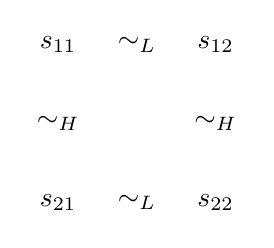
\begin{tikzpicture}
  \node (n1) {$s_{11}$};
  \node (n2) [right of= n1] {$\sim_L$};
  \node (n3) [right of= n2] {$s_{12}$};
  \node (n10) [below of= n1] {$\sim_H$};
  \node (n11) [below of= n3] {$\sim_H$};
  \node (n4) [below of= n10] {$s_{21}$};
  \node (n5) [right of= n4] {$\sim_L$};
  \node (n6) [right of= n5] {$s_{22}$};
\end{tikzpicture}

% figure 2 here

\begin{definition}[Robust declassification]  
\begin{equation*}
  \llbracket s_{11} \rrbracket \approx_L \llbracket s_{21} \rrbracket \ \land \text{ relevant inputs} \Rightarrow \llbracket s_{12} \rrbracket \approx_L \llbracket s_{22} \rrbracket 
\end{equation*}
\end{definition}


\begin{definition}[Transparent endorsement]
\begin{equation*}
  \llbracket s_{11} \rrbracket \approx_H \llbracket s_{12} \rrbracket \ \land \text{ relevant inputs} \Rightarrow \llbracket s_{21} \rrbracket \approx_H \llbracket s_{22} \rrbracket
\end{equation*}  
\end{definition}  

RD + TE ="nonmalleable informationi flow"

\paragraph{Where do $\bigtriangleup$ and $\bigtriangledown$ come from?}\ 

FLAM (Arden et al. CSF'15)
\begin{enumerate}
    \item labels are principals
    \item primitive principals (Alice, Bob, p, q, $\ldots$)
    \item prinicpal projections ($p^{\leftarrow}$ integrity projection, $p^{\rightarrow}$ confidentiality)
    \item joins and meets on principals $p \land q$ (reads as: powers of both $p$ and $q$), $p \lor q$.
      \begin{equation*}
        \forall p,q. p \land q \succeq p \succeq p \lor q
      \end{equation*}
where $\succeq$ is a trust ordering. Least powerful principal is $\bot$; most powerful is $\top$. %see figure 3
\end{enumerate}

A normal form for principals is $A^{\leftarrow} \land B^{\rightarrow}$, where $A,B$ are CNF expressions over primitive principals. Then $\bigtriangleup$ and $\bigtriangledown$ are defined as:

\begin{align*}
  \bigtriangleup (A \la \land B \ra) &= A \ra \land T \la \\
  \bigtriangledown (A \la \land B \ra) &= B \la \\
  \text{Reflection:} \refl (A \la \land B \ra) &= B \la \land A \ra                                         
\end{align*}


If something has label $l \not\sqsubseteq \refl l$, we can't downgrade it nonmalleably.
%figure 4 here

\section{Hardware security}
\begin{tabular}{|c|}
Modern systems \\
\hline
app code \\
\hline
libraries \\ 
\hline
OS \\
\hline
ISA \\ 
\hline
$\mu$ architecture \\
\end{tabular}{|c|}

Correctness and security depend on having contracts between these different layers. 

Classic specifications do not work (Meltdown, spectre). Contracts should capture information flow (hyperproperties)

Contracts should be compositional

%figure 5 here
Mandatory vs. discretionary access control

Example
\begin{lstlisting}[mathescape]
if h_1 then
    h_2 := l_1 // pulls l_1 into cache
else 
    h_2 := l_2
l_3 := l_1 // false if h_1 = true
\end{lstlisting}

Timing update to $l_3$ teaches value of $h_1$.

Zhang/PLDI'12: ISA/M-arch contract that rules out timing channels (in addition to previously discussed leakage)
Zagieboylo/CSF'19: detailed ISA contract for realistic ISA supporting nonmalleable downgrading

Consider imperative language IMP where each command has a \emph{read label} and a \emph{write label}.
Read label $l_r$ bounds influences on time taken by instruction
Write label $l_w$ is a lower bound on effects instruction has on $\mu$-architecture state
\begin{tabular}{|c|}
\hline
ISA
$\quad$ register \\
\hline
$\mu$-arch \\
$\quad$ cache \\
$\quad$ TLB \\
$\quad \ldots$ \\
\hline
\end{tabular}

Define two types of semantics
architecturlar semantcs (like SOS, $c,\gamma \longrightarrow c',\gamma'$)
$\mu$-arch semantics: $c,\gamma,E,G \longrightarrow c',\gamma',E',G'$

where $E$ =  the microarchitecture state, $G$ is global (wall-clock) time.
 
read-label property: Given command $c_[l_r,l_w]$
$(\forall x \in vars(c) . \gamma_1(x) = \gamma_2(x)) \land E_1 ~_{l_r} E_2) \land c_[l_r,l_w],\gamma_i,E_i,G \longrightarrow c_i,\gamma_i',E'_i,G_i)  \Rightarrow G_1 = G_2$ for $i \in 
\{1,2\}$

write-label property: $l_w \not\sqsubseteq l \land c_{[l_r,l_w]}, \gamma,E,G \longrightarrow c', \gamma',E',G' \Rightarrow E ~_l E' $

Single-step noninterference
$(\gamma_1 ~-l \gamma_2 \land E_1 ~_l E_2 \land c_{l_r,l_w},\gamma_i,E_i,G_i \longrightarrow c_i,\gamma'_i,E'_i,G_i') \Rightarrow E'_1 = E'_2$

Hardware satisfying these three porperties can reason about information flow for software/hardware composition

\begin{lstlisting}[mathescape]
if h_1 then
    h_2 := l_1[L,H] // pulls l_1 into cache
else 
    h_2 := l_2[L,H]
l_3 := l_1[L,L] // false if h_1 = true
\end{lstlisting}
$h_1$ flows into assignment $h_2$ of $l_1$

\section{HDLs}
(Hardware description language)

How do you build \emph{efficient} hardware that \emph{verifiably} satisfies security properties?
Use SecVerilog = Verilog + security labels

\begin{itemize}
\item Threat model = adversary can see all public memory at every clock cycle.

\item Partition cache statically

\item Annotations on variables (possibly functions)
  
\end{itemize}

\emph{Soundness:} at each clock tick, no H information leaks to a L variable.
  
See slides for the rest.



\end{document}

%%% Local Variables:
%%% mode: latex
%%% TeX-master: t
%%% End:
